%!TEX root = ../Report.tex
\chapter{Implementação}
\label{chp:implement}
Esta secção apresenta a implementação das ferramentas acima mencionadas e a forma como estas foram utilizadas no contexto do projeto, desde a sua interação com outras ferramentas até aos seus benefícios para a solução. As seguintes subseções falam, em primeiro lugar, da camada de dados e como esta está organizada de modo a suportar o armazenamento de dados necessitado para o projeto.\newline
Em segundo lugar, descreve a camada de processamento e como a comunicação e a troca de dados é feita entre as várias secções da plataforma, como por exemplo, entre o frontend e a base de dados.\newline
Por fim descreve o frontend e como este está estruturado de modo a cumprir os objetivos que foram definidos para o projeto e também fala acerca dos nós/APUs, como estes estão configurados e como eles são acedidos e reconfigurados pelo utilizador da plataforma que pretende realizar experiências.

\section{Camada de dados}
Nesta secção vamos discutir com detalhe a implementação da camada de dados. Em primeiro lugar, demonstramos o modelo de dados da base de dados.\newline
No bloco dos utilizadores, temos as seguintes tabelas:
\begin{itemize}
    \item \textbf{Profile} – esta tabela modela um utilizador e as suas informações;
    \item \textbf{Experience} – esta tabela modela uma experiência como por exemplo a sua data de início e de fim;
    \item \textbf{APU\_Config} - define a configuração a fornecer a APU para uma dada experiência;
    \item \textbf{APU} – tabela que contém a informação acerca de cada APU da rede como por exemplo o IP;
    \item \textbf{Role} – cada utilizador pode ser de vários roles como por exemplo “Advanced” e “Beginner”
\end{itemize}
\begin{figure}[!ht]
    \centering
    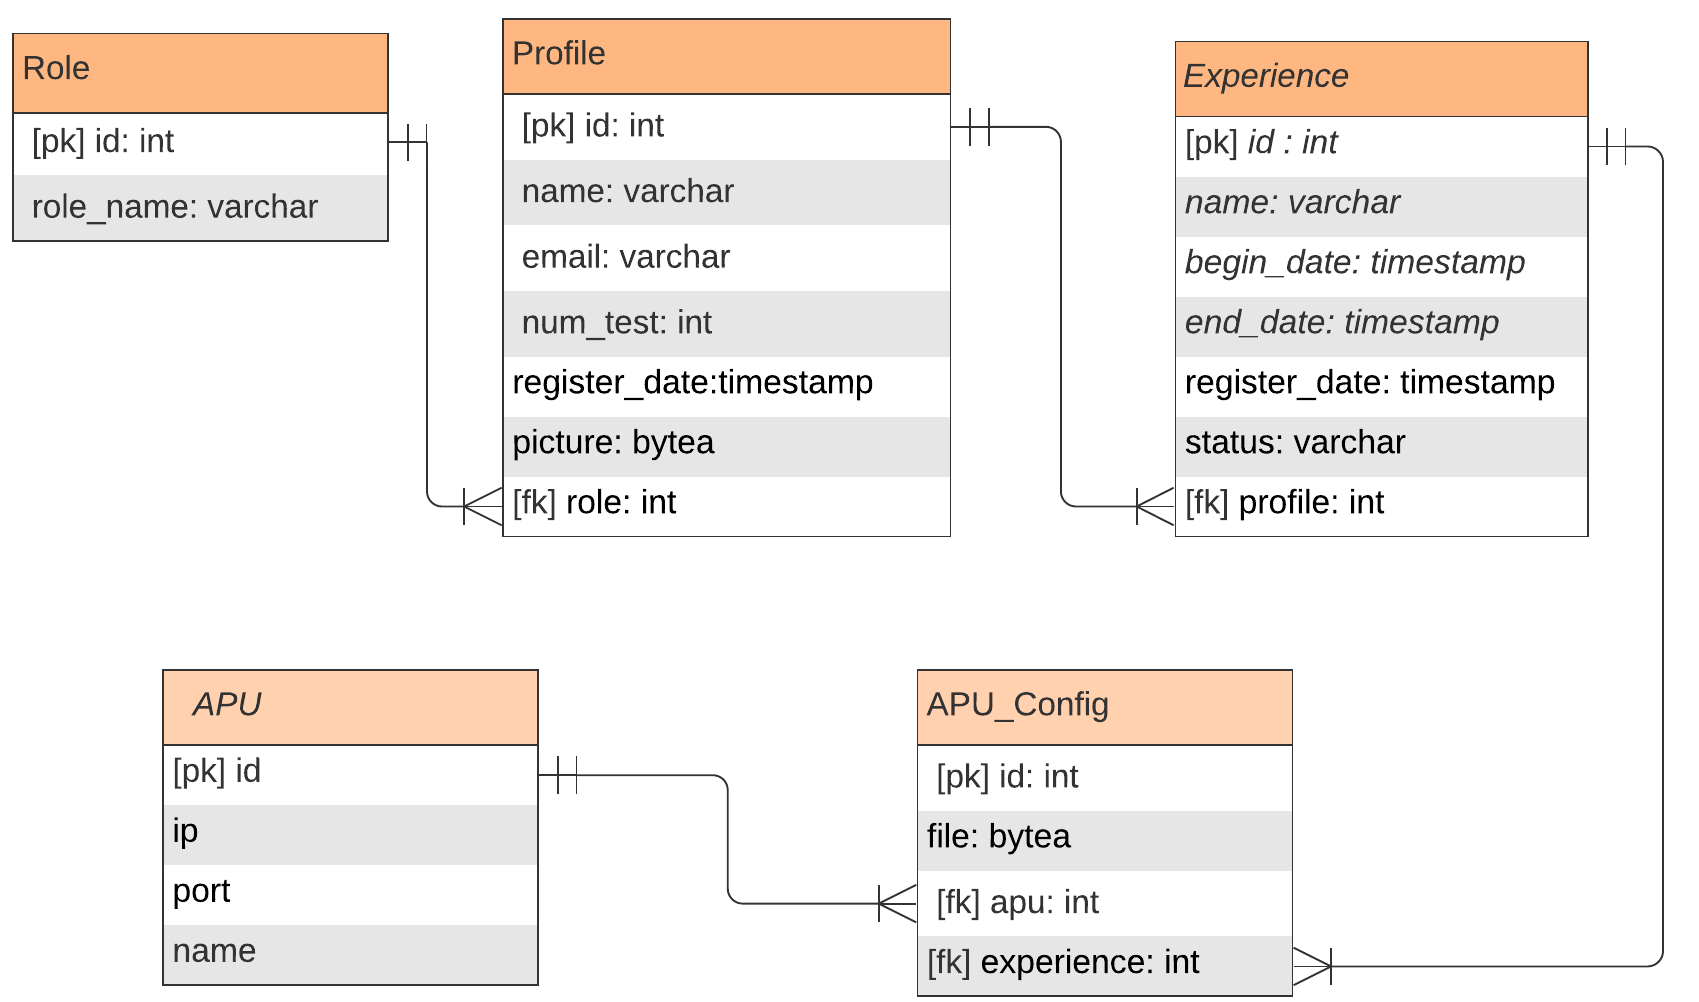
\includegraphics[width=0.75\textwidth, height=0.347\textheight]{images/data_model.png}
    \caption{Modelo de dados (bloco do utilizador)}
    \label{fig:dataModel}
\end{figure}
\section{Camada de processamento}
Esta secção apresenta o servidor principal da plataforma construído utilizando a framework Flask. Esta camada é responsável pela gestão do sistema, prover e receber dados do FrontEnd, consumir e atualizar a base de dados. Além de interagir com a Base de Dados, esta camada também interage com as APUs, inicializando automaticamente experiências e atuando como um proxy para disponibilizar informações das APUs em tempo real.
\begin{figure}[!ht]
    \centering
    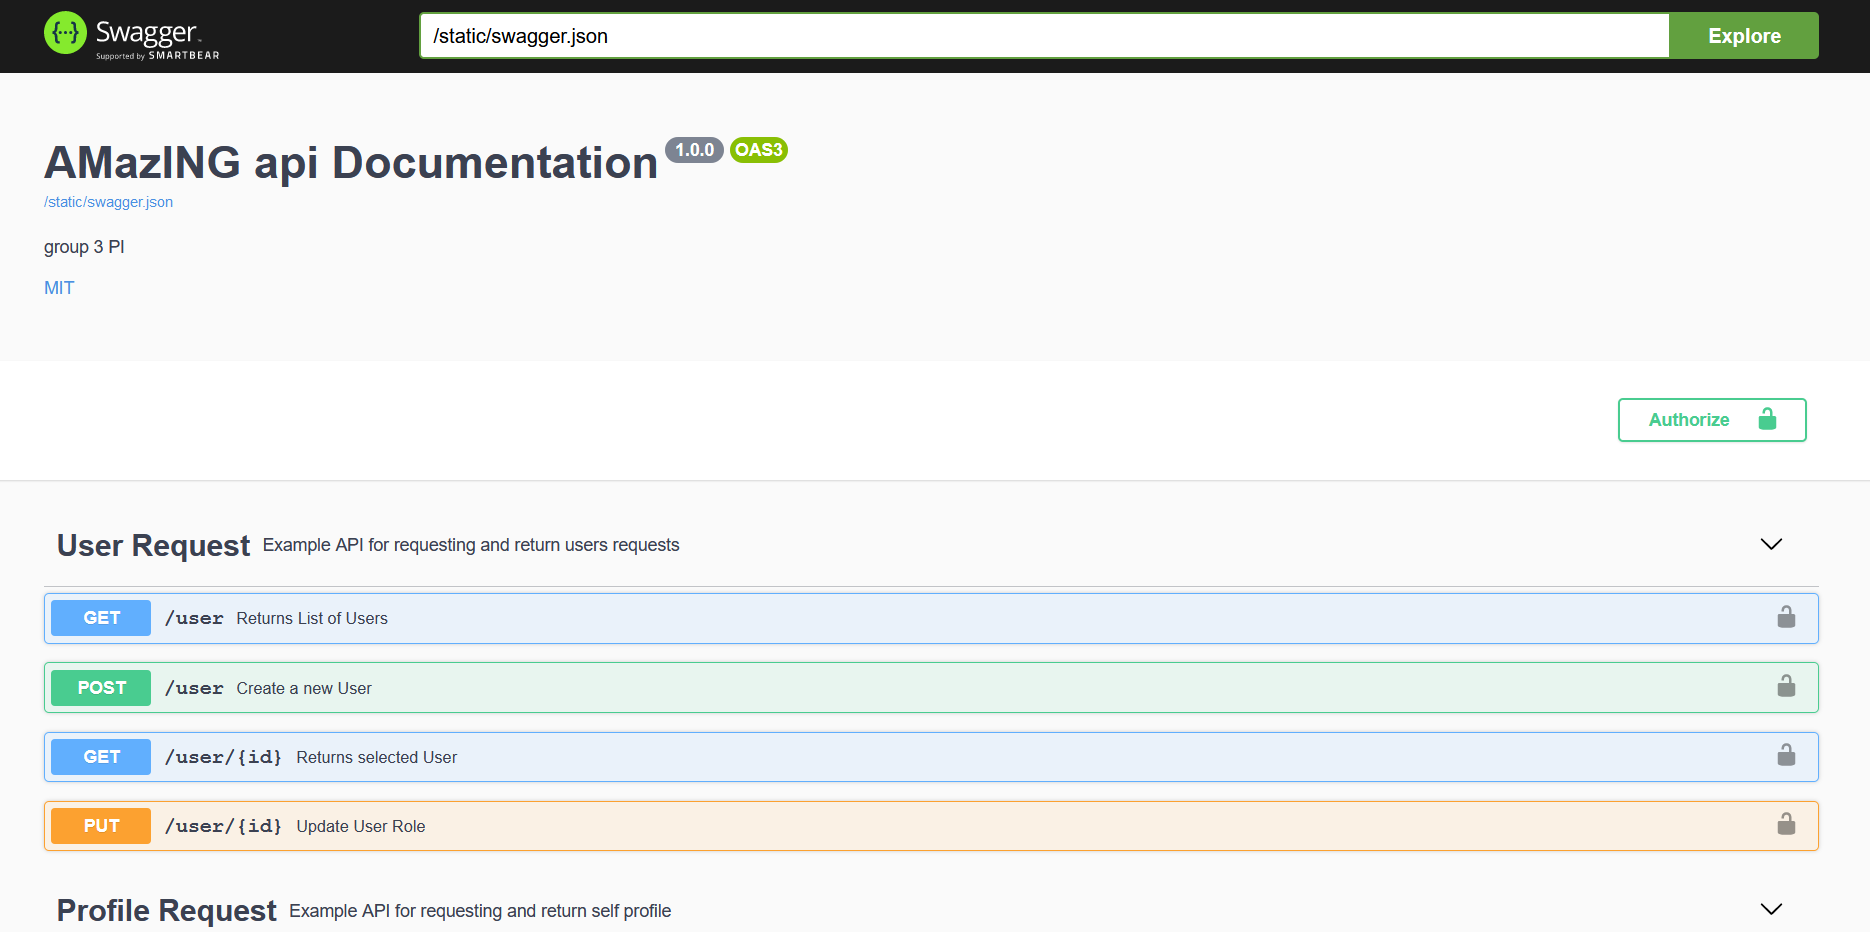
\includegraphics[width=0.9\textwidth]{images/swagger.png}
    \caption{Fragmento da documentação do Servidor utilizando o swagger}
    \label{fig:swagger}
\end{figure}

\section{Fluxo de dados}
Esta secção, contém os fluxos de informação que passam ou se iniciam pelo servidor.\newline
Inicializando pelos pedidos tipo GET, que buscam informação da base de dados e retornam os dados , tratada de acordo com o necessário. Este tipo de operação não realiza alteração na informação da base de dados.
\begin{figure}[!ht]
    \centering
    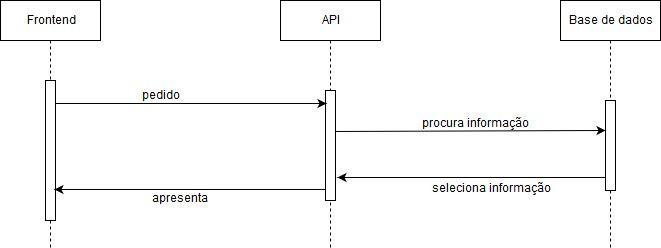
\includegraphics[width=\textwidth]{images/fluxo1.jpg}
    \caption{Fluxo de comunicação para o método GET}
    \label{fig:get}
\end{figure}
\begin{figure}[!ht]
    \centering
    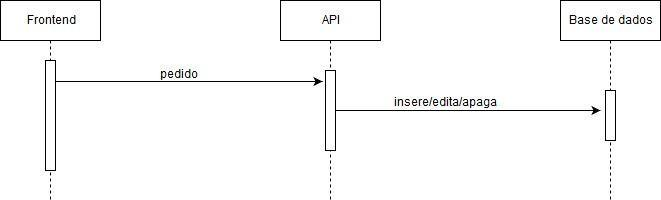
\includegraphics[width=\textwidth]{images/fluxo2.jpg}
    \caption{Fluxo de comunicação para os métodos POST, PUT e DELETE}
    \label{fig:post}
\end{figure}
\newpage
\begin{figure}[!ht]
    \centering
    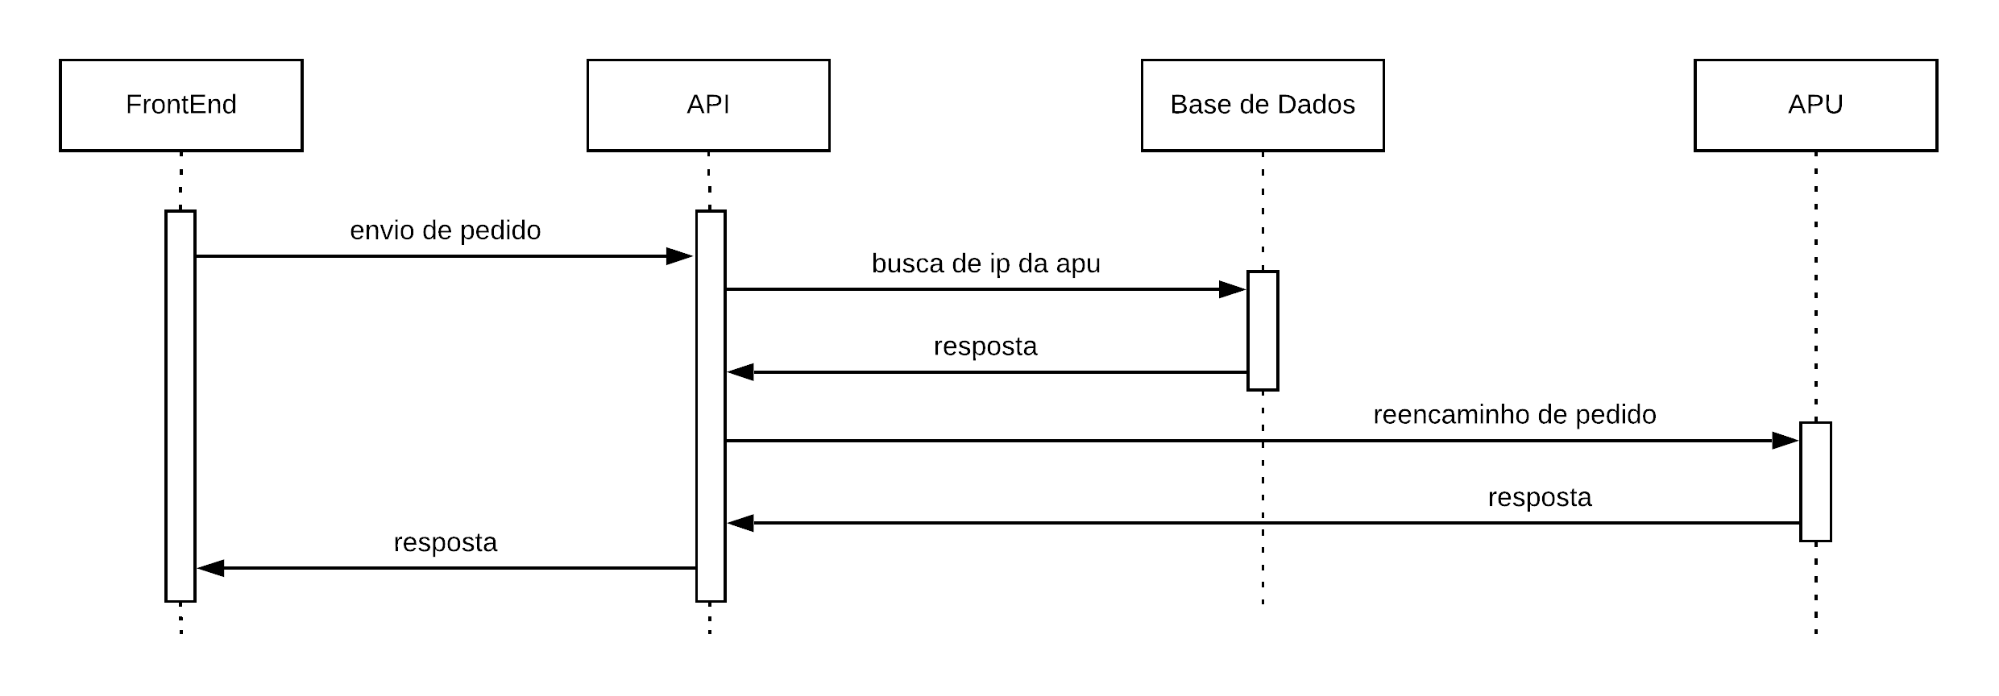
\includegraphics[width=\textwidth]{images/fluxo3.png}
    \caption{Fluxo de comunicação Proxy, para os métodos GET e POST}
    \label{fig:proxy}
\end{figure}
\begin{figure}[!ht]
    \centering
    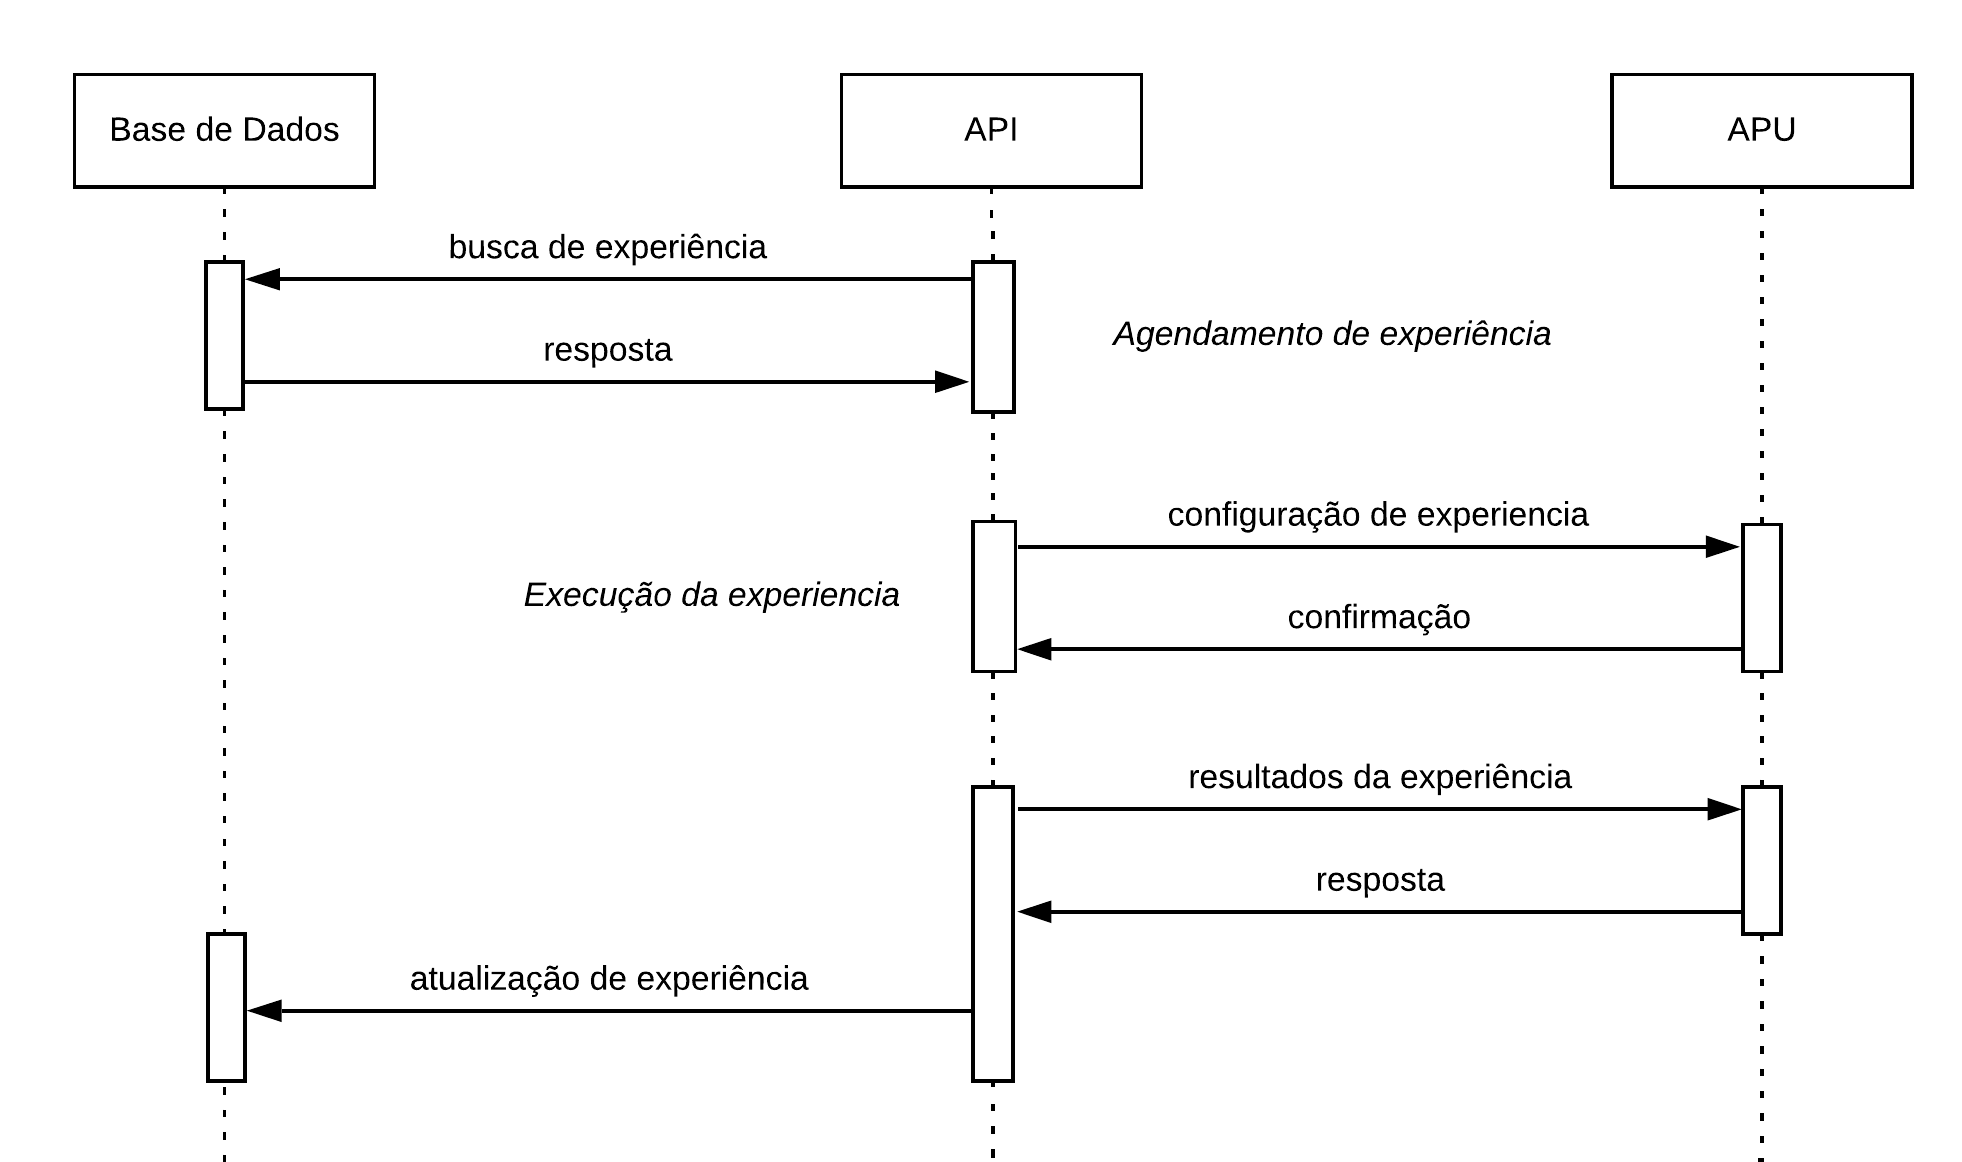
\includegraphics[width=\textwidth]{images/fluxo4.png}
    \caption{Fluxo de comunicação Proxy, para os métodos GET e POST}
    \label{fig:agendamento}
\end{figure}
\section{Frontend}
INSERIR TEXTO

\section{Nós/APU}
ISERIR


\newpage
\hfill\break